\Chapter{Alkalmazásbeli példa}

\Section{A kód}
\SubSection{Alapkoncepció}
Először egy egyszerű Python applikációba szerettem volna megvalósítani a megjelenítést és magát az egész projektet. Ehhez a TKInter nevű könyvtárat szándékoztam használni, állítható értékekkel, hogy megfigyeljem melyik érték kombinációval a legcélszerűbb a kép beolvasása és az adatok kinyerése onnan. Leegyszerűsített használatra, csak akkordokkal foglalkozva a kék színnel ábrázolt akkordokat szándékoztam kinyerni a képből. Végül a csúszkákat félretéve manuálisan írtam át az értékeket, egy numpy tömbbe csomagoltam be ezeket. Ezek az értékek kellettek ahhoz, hogy meghatározzam a cv2-nek, hogy milyen színskálába szeretném kiszedni az akkordokat. 
\par
Kísérleteztem azzal, hogy ha változtatom a skálát, akkor milyen pontossággal tudja visszaadni csak az akkordokat(amik kékkel vannak feltüntetve) a képről. Az volt a terv, hogy akkor ez mint bemeneti kép lesz majd kiolvasva a képből az OCR segítségével. Ehhez az kellett, hogy a megfelelő spektrumba legyen a program színhatára, amit ki tud olvasni zajmentesen, mivel a kották egységes kék színnel vannak kezelve akkordok terén, ezért nem kell egyáltalán változó értékű tömböket használni a színskála beállításához.
\par

\SubSection{Kimeneti példák}
A következőkben áttértem jupyter-notebookra, hogy lehessen szétbontani, és emészthetőbbé kialakítani a kódot.

\begin{python}
this_img = cv2.imdecode(numpyarray, cv2.IMREAD_UNCHANGED)	
\end{python}



\SubSection{Tesseract használata}
A tesseract nevezetű OCR szoftvert használom a karakterfelismerésre a dolgozatban, nevezetesen a pytesseract függvénykönyvtárat. Ez alapvetően a Google OCR motorja, amit implementáltak python környezetben. Önmagába álló szkriptként is használható, és széles körben felismer különböző kiterjesztésű képeket, mint például a jpeg, png, gif, bmp, tiff és egyéb másokat, habár ugyanúgy megvannak a korlátai is, amiről majd később térek ki részletesebben. Elsőként mivel hogy különálló maga a program ezért PATH-ba kellett helyezni, amivel sajnos meggyűlt a baj, mivel hogy nem ismerte fel az operációs rendszer. Így a következőképpen oldottam meg, hogy használható legyen:
\begin{python}
	import pytesseract
	
	local_path =  r'C:\Program Files\Tesseract-OCR\tesseract.exe'
	pytesseract.pytesseract.tesseract_cmd = local_path
\end{python}
A lokális környezetbe való fejlesztés erejéig volt használatba ez az elérési útvonal. A függvénykönyvtárnak az image to string nevű metódusát használtam arra, hogy a képből szöveg váljon. Paraméterként megadható, hogy ugye mely képekből kell a szöveget kiolvasni, és többek között, amit használtam én is az a nyelv megadása, valamint konfigurációt is meg tudtam adni. A pontosság az elején zavaró volt, mert túlságosan zajos volt a kép sokszor, ahhoz, hogy az OCR megfelelően ki tudja venni, hogy mely karakterről is van szó. Ehhez az egyik megolás az volt, hogy jobban lehessen manipulálni a bemeneti képet, amivel dolgozik a Tesseract.
\par
\SubSection{Kottafeldolgozás}
A kottákat, mint képeket (legyen az jpeg, vagy png, vagy bármilyen más képformátum) beolvassa az opencv könyvtár imdecode metódusa
\begin{python}
stream = open(im_path, "rb")
bytes = bytearray(stream.read())
numpyarray = np.asarray(bytes, dtype=np.uint8)
this_img = cv2.imdecode(numpyarray, cv2.IMREAD_UNCHANGED)
\end{python}
Megnyitom olvasásra, és egy stream-be tárolom le, ahol mátrixszerűen letárolja a numpy. Itt többek között megadható, az hogy milyen kódolással tárolja le. Az imdecode

\begin{figure}[h]
	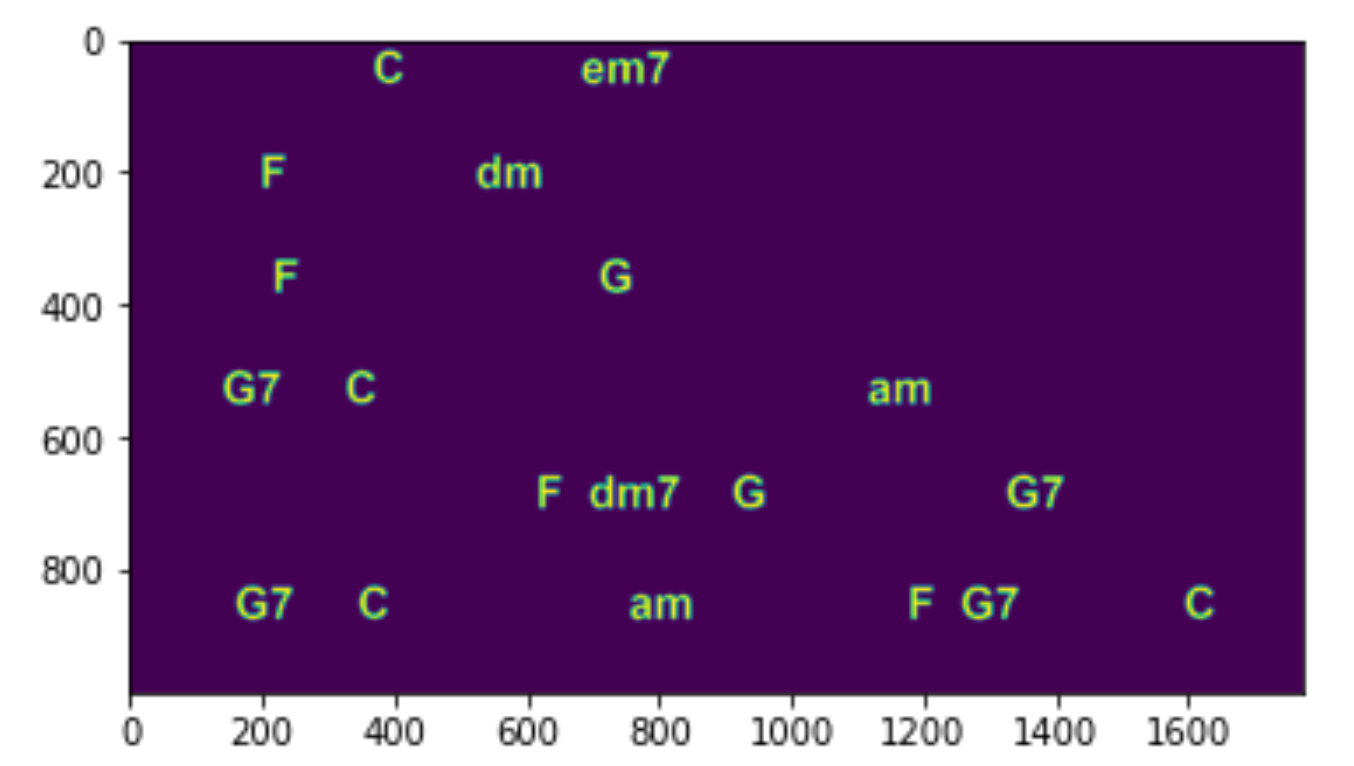
\includegraphics[scale=0.5]{images/output_justchords.png}
	\caption{Kotta akkordjai}
	\label{fig:output2}
\end{figure}

\begin{figure}[h]
	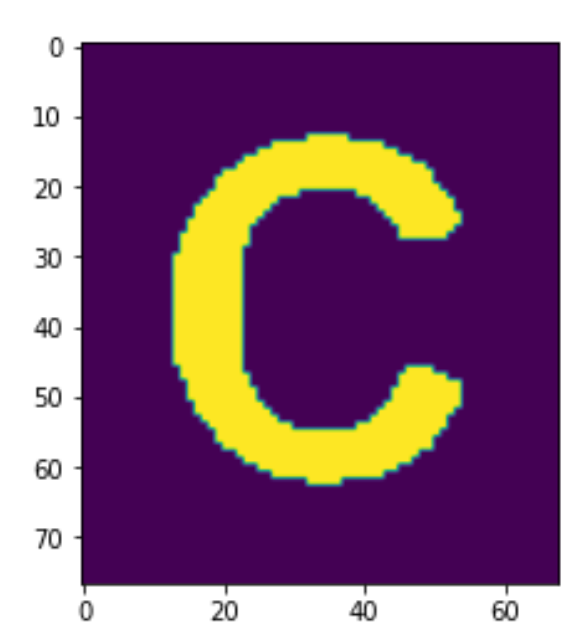
\includegraphics[scale=0.5]{images/output_single_character.png}
	\caption{A kotta egyik akkordja}
	\label{fig:output3}
\end{figure}

\begin{figure}[h]
	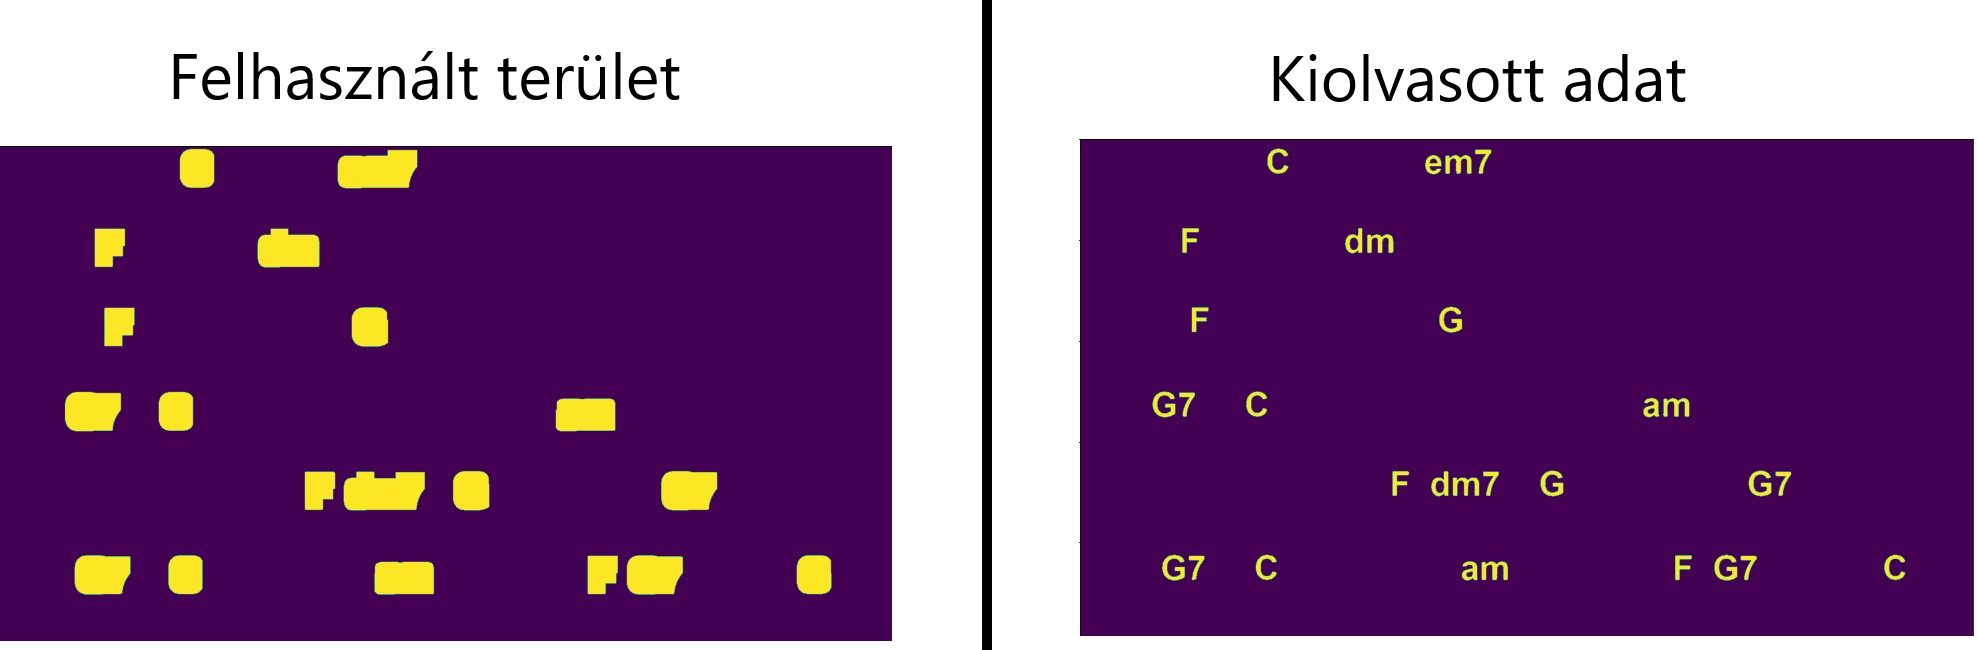
\includegraphics[scale=0.3]{images/misc/chord_overlay.jpg}
	\caption{A terület és a kiolvasott adat, amit a program lát}
	\label{fig:output4}
\end{figure}

\Section{Lekérdezések kezelése}
Ebben a szekcióban lesz taglalva, hogy miként valósult meg az rdf egyes szerializációjának a betöltése és lekérdezése.

\SubSection{SPARQL}

Az RDF/XML féle szerializációval készítettem egy olyan programot ami betölti, majd feldolgozza az xml-t, hogy lekérdezéseket lehessen írni belőle. A következő lekérdezés kilistázza azokat az akkordokat, amelyek megtalálhatók a kottában.

\begin{python}
query_string_all_chord = """
    SELECT DISTINCT?o
    WHERE {
        ?s segment:note ?o .
        ?s ?p ?o .
    }
"""

q_res = g.query(query_string_all_chord)
for row in q_res:
    print(f"Akkord: {row.o}")
\end{python}
\begin{verbatim}
OUTPUT:
Akkord: C
Akkord: em7
Akkord: F
Akkord: dm
Akkord: F/G
Akkord: G
Akkord: G7
Akkord: am
Akkord: dm7
\end{verbatim}

Lekérdezhető az is, hogy milyen akkordhoz milyen szövegrész tartozik, vagy fordítva, ha szeretném megtudni azt, hogy egy szövegrészhez milyen akkord társul. Ehhez szükséges volna egy olyasfajta validáció, ami először végigpásztázza, hogy a kapott input az pontosan úgy megtalálható e a szerializált xml-ben, vagy sem.

\begin{python}
query_string_one_chord = '''
    SELECT ?s ?p ?o ?p1 ?o1
    WHERE {
        ?s ?p 'C' .
        ?s ?p ?o .
        ?s segment:text ?o1 .
        ?s ?p1 ?o1 .
    }
'''

q_res = g.query(query_string_one_chord)
for row in q_res:
    print(f"{row.o}\n {row.o1}")
\end{python}
\begin{verbatim}
OUTPUT:
C
 Tied a dicsőség, 
C
 mas, 
C
 mas, 
C
 mas!
\end{verbatim}

\SubSection{Szimpla XML feldolgozása}

\begin{python}
tree = ET.parse(source='sheetparser.xml')

...

if child.tag == "segment":
	...
	
  if position_substring in line:
    occ = line.count(position_substring)
    ind_of_line = (line.replace(position_substring, '___', occ) + text)
      .find(position_substring)
    line.replace('___', position_substring, occ)
    line += text
  else:
    line += text
    ind_of_line = line.index(position_substring)
	            
     ...
     
  if segment_num.count(child.attrib['id']) > 0:
    ret += "\n"
    su += ret + line.replace(r'\n', "\n")
    ret, line = '', ''
    ind, notes = [], []
    count, sum_of_ind = 0, 0
\end{python}

--

\begin{figure}[h]
	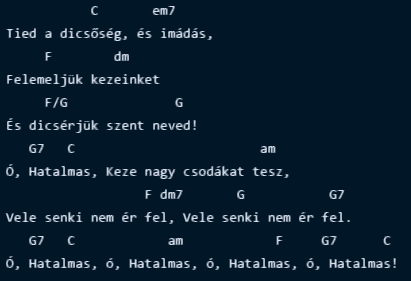
\includegraphics[scale=1]{images/output_tied.png}
	\caption{Az xml beolvasó program kimenete}
	\label{fig:output1}
\end{figure}